% Chapter 2
\chapter{TỔNG QUAN VỀ VẤN ĐỀ NGHIÊN CỨU}
\label{Chapter2}

Chương này tổng quan về các khái niệm nền tảng và tình trạng nghiên cứu, gồm: IoT và thách thức an toàn thông tin, hệ thống IDS, Federated Learning, các tấn công poisoning/backdoor, phương pháp phòng thủ hiện có, và Digital Twin trong FL-IoT.

\section{Giới thiệu về Internet of Things (IoT)}

\subsection{Khái niệm và kiến trúc IoT}
Internet of Things (IoT) là một mạng lưới các đối tượng vật lý (thiết bị, phương tiện, tòa nhà và các vật phẩm khác) được nhúng cảm biến, phần mềm, và khả năng kết nối mạng, cho phép các đối tượng này thu thập và trao đổi dữ liệu. Khái niệm IoT đã phát triển từ những nghiên cứu ban đầu trong thập niên 1990 và sau đó được mở rộng nhờ sự phát triển mạnh mẽ của công nghệ kết nối không dây, cảm biến giá rẻ, và điện toán đám mây.

Kiến trúc IoT thường được chia thành ba lớp chính:

\textbf{Lớp Perception (Cảm nhận):} Đây là lớp thấp nhất trong kiến trúc IoT, bao gồm các cảm biến và thiết bị thu thập dữ liệu từ môi trường vật lý. Các cảm biến này có thể đo nhiều loại dữ liệu như nhiệt độ, độ ẩm, chuyển động, hình ảnh, âm thanh, lưu lượng mạng, và nhiều tham số khác. Tại lớp này, dữ liệu được thu thập sơ bộ, đôi khi được tiền xử lý trước khi chuyển lên lớp cao hơn.

\textbf{Lớp Network (Mạng):} Lớp này đảm bảo kết nối và truyền tải dữ liệu giữa các thiết bị IoT và các hệ thống xử lý. Các giao thức kết nối đa dạng tùy thuộc vào yêu cầu về băng thông, độ trễ, và tiêu thụ năng lượng: Wi-Fi, Bluetooth, Zigbee, LoRaWAN, 4G/5G, và các giao thức chuyên dụng khác. Lớp mạng cũng đảm bảo các dịch vụ định tuyến, bảo mật, và quản lý kết nối.

\textbf{Lớp Application (Ứng dụng):} Lớp cao nhất nơi dữ liệu từ IoT được xử lý, phân tích, và sử dụng cho các mục đích cụ thể. Các ứng dụng IoT có thể trong nhiều lĩnh vực như nhà thông minh (điều khiển đèn, nhiệt độ), y tế thông minh (theo dõi bệnh nhân, thiết bị y tế), giao thông thông minh (quản lý đèn tín hiệu, giám sát giao thông), công nghiệp 4.0 (giám sát sản xuất, bảo trì dự đoán), và nông nghiệp chính xác (theo dõi đất, thời tiết, tự động tưới).

\begin{figure}[H]
    \centering
    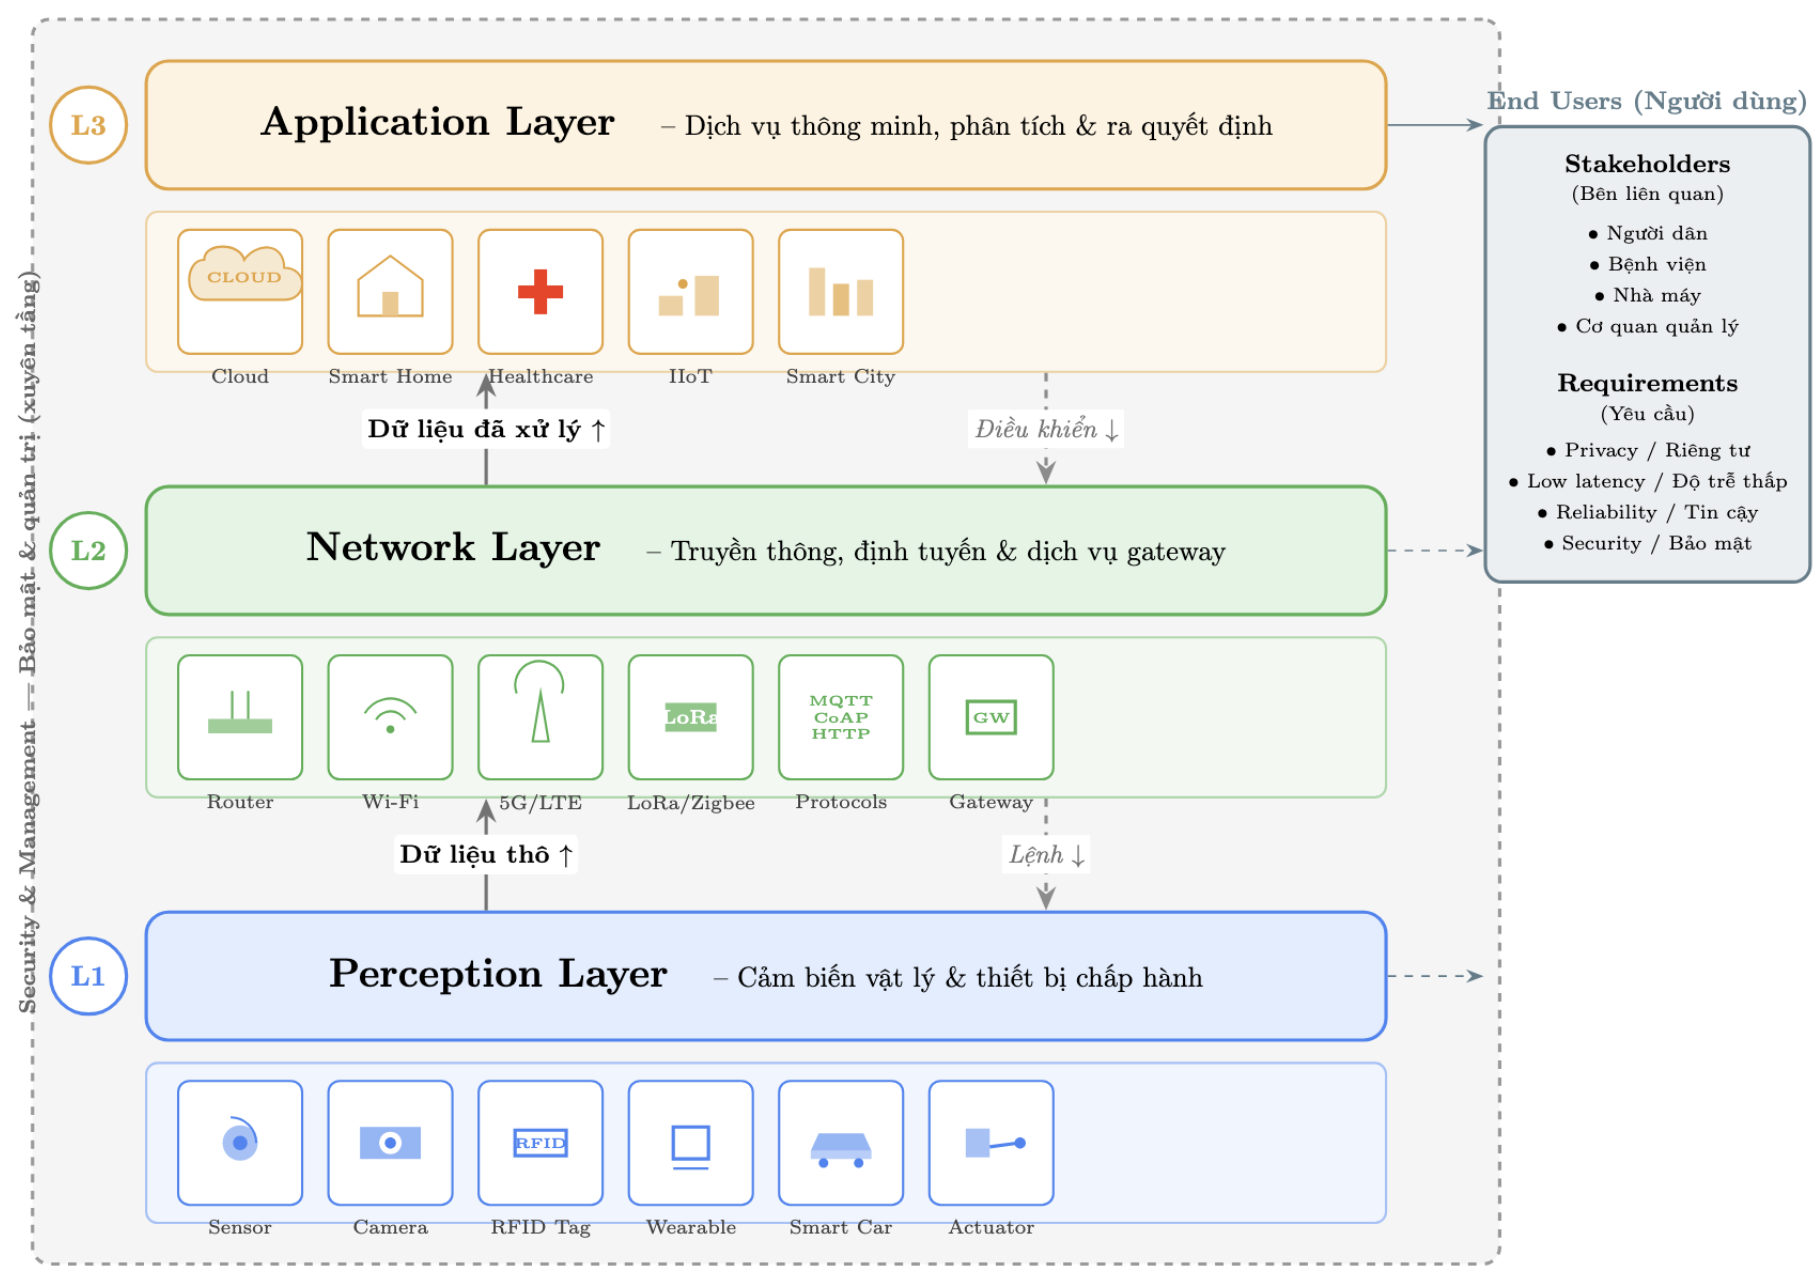
\includegraphics[width=0.85\linewidth]{Figures/fig_2_1_kien_truc_iot_3_lop.png}
    \caption{Kiến trúc IoT 3 lớp}
\end{figure}

Các thiết bị và giao thức IoT phổ biến hiện nay rất đa dạng. Về thiết bị, có thể kể đến: cảm biến môi trường (nhiệt độ, độ ẩm, áp suất), thiết bị giám sát (camera, microphone), thiết bị đeo (smartwatch, fitness tracker), thiết bị gia dụng thông minh (tủ lạnh, máy giặt, điều hòa), thiết bị công nghiệp (robot, máy móc tự động), và xe thông minh. Về giao thức, có các giao thức tầm ngắn năng lượng thấp như Zigbee, Z-Wave, LoRaWAN cho các ứng dụng cảm biến; Bluetooth và BLE cho thiết bị đeo và gia dụng; Wi-Fi cho các ứng dụng băng thông cao như camera giám sát; và mạng di động 4G/5G cho các ứng dụng cần độ phủ sóng rộng.

\subsection{Thách thức an toàn thông tin trong IoT}
Internet of Things mang lại nhiều lợi ích nhưng cũng đối mặt với nhiều thách thức an toàn thông tin đặc thù. Các đặc tính của IoT tạo điều kiện cho các mối đe dọa an toàn thông tin mới hoặc làm gia tăng mức độ nghiêm trọng của các mối đe dọa đã tồn tại.

\textbf{Đặc tính của IoT:}

IoT có nhiều đặc tính khác biệt với các hệ thống truyền thống. \textbf{Số lượng thiết bị lớn}: Hệ thống IoT có thể bao gồm hàng triệu thiết bị phân tán trên diện tích rộng. \textbf{Tài nguyên hạn chế}: Nhiều thiết bị IoT có năng lượng, bộ nhớ, và khả năng xử lý hạn chế do yêu cầu kích thước nhỏ, tiêu thụ năng lượng thấp, và chi phí rẻ. \textbf{Môi trường không an toàn}: Các thiết bị IoT thường được triển khai trong môi trường công cộng, dễ bị tiếp cận vật lý để thao túng hoặc tấn công. \textbf{Kết nối đa dạng}: Sự kết nối thông qua nhiều giao thức khác nhau tạo ra nhiều điểm tấn công tiềm năng.

\textbf{Các mối đe dọa an toàn thông tin trong IoT:}

Các mối đe dọa an toàn thông tin trong IoT rất đa dạng và có thể được phân loại theo nhiều tiêu chí. Theo lớp tấn công: \textbf{Tấn công vật lý}: tiếp cận trực tiếp thiết bị để thao túng, sao chép dữ liệu, hoặc thay thế thiết bị giả mạo. \textbf{Tấn công mạng}: tấn công vào giao thức và kết nối mạng như đánh giá lại, chèn gói tin, từ chối dịch vụ (DoS/DDoS). \textbf{Tấn công phần mềm}: khai thác lỗ hổng trong phần mềm, firmware, hoặc hệ điều hành của thiết bị IoT. \textbf{Tấn công mã hóa}: tấn công vào cơ chế mã hóa và xác thực để truy cập trái phép dữ liệu hoặc hệ thống.

Theo mục đích: \textbf{Tấn công phát hiện xâm nhập}: cố gắng phát hiện và thu thập thông tin về hệ thống IDS để lẩn tránh. \textbf{Tấn công lấy cắp dữ liệu}: đánh cắp dữ liệu cảm biến hoặc thông tin cá nhân từ thiết bị IoT. \textbf{Tấn công từ chối dịch vụ}: làm cho hệ thống không thể phục vụ người dùng hợp pháp. \textbf{Tấn công điều khiển}: chiếm quyền điều khiển thiết bị hoặc hệ thống để thực hiện hành vi nguy hiểm.

\textbf{Yêu cầu bảo vệ quyền riêng tư dữ liệu:}

Dữ liệu từ thiết bị IoT thường chứa thông tin nhạy cảm về hành vi người dùng, hoạt động gia đình, hoặc dữ liệu y tế. Việc bảo vệ quyền riêng tư dữ liệu IoT là một yêu cầu quan trọng, cả về mặt pháp lý và đạo đức. Các quy định pháp lý như GDPR tại Châu Âu, CCPA tại Mỹ, và các quy định về bảo vệ dữ liệu cá nhân khác hạn chế việc thu thập và xử lý dữ liệu cá nhân mà không có sự đồng ý của người dùng. Hệ thống phát hiện xâm nhập truyền thống thường yêu cầu tập trung hóa dữ liệu để huấn luyện mô hình, điều này có thể xung đột với các quy định về quyền riêng tư và tạo ra rào cản pháp lý cho việc triển khai.

\section{Hệ thống phát hiện xâm nhập mạng (Intrusion Detection System)}

\subsection{Khái niệm và nguyên lý hoạt động của IDS}
Hệ thống phát hiện xâm nhập (Intrusion Detection System - IDS) là một thiết bị hoặc ứng dụng phần mềm giám sát mạng hoặc hệ thống để tìm các hoạt động vi phạm chính sách hoặc hoạt động bất thường. IDS là một thành phần quan trọng trong hệ thống an toàn thông tin, đóng vai trò tuyến phòng thủ chủ động để phát hiện các cuộc tấn công hoặc hành vi bất thường kịp thời.

\textbf{Quy trình hoạt động cơ bản của IDS:}

Quy trình hoạt động cơ bản của IDS gồm các bước sau:

\textbf{Bước 1: Thu thập dữ liệu.} IDS thu thập dữ liệu từ mạng hoặc hệ thống thông qua nhiều nguồn khác nhau như network packets, system logs, process activities, và các sự kiện hệ thống khác. Dữ liệu thu thập được bao gồm thông tin về địa chỉ IP, cổng, giao thức, nội dung gói tin, thời gian, và nhiều thông tin khác.

\textbf{Bước 2: Phân tích dữ liệu.} Dữ liệu thu thập được phân tích theo các quy tắc hoặc mô hình học được. Phân tích có thể được thực hiện theo thời gian thực (real-time) để phát hiện ngay lập tức các cuộc tấn công, hoặc được thực hiện theo thời gian rời rạc (offline) để phân tích lại các log và phát hiện các cuộc tấn công đã xảy ra.

\textbf{Bước 3: Phát hiện các dấu hiệu.} Từ việc phân tích dữ liệu, IDS phát hiện các dấu hiệu của tấn công hoặc hành vi bất thường. Các dấu hiệu này có thể là các mẫu tấn công đã biết (signature), các hoạt động bất thường so với hành vi bình thường, hoặc các kết hợp của cả hai.

\textbf{Bước 4: Kích hoạt cảnh báo hoặc phản hồi.} Khi phát hiện dấu hiệu tấn công hoặc hành vi bất thường, IDS kích hoạt cảnh báo hoặc phản hồi tự động. Cảnh báo được gửi cho quản trị viên qua email, SMS, hoặc các kênh khác. Phản hồi tự động bao gồm chặn kết nối, cô lập hệ thống, hoặc thực hiện các hành động phòng thủ khác.

\textbf{Vai trò của IDS trong hệ thống an toàn thông tin:}

IDS có ý nghĩa quan trọng trong hệ thống an toàn thông tin như một lớp phòng thủ chủ động. Khác với tường lửa (firewall) chỉ chặn các kết nối dựa trên quy tắc được định nghĩa trước, IDS có thể phát hiện các cuộc tấn công mới và các hành vi bất thường chưa có trong quy tắc. IDS kết hợp với các thành phần an toàn khác như tường lửa, hệ thống chống virus, và hệ thống giám sát để tạo thành một hệ thống an toàn toàn diện.

\subsection{Phân loại IDS}
IDS có thể được phân loại theo nhiều tiêu chí khác nhau tùy thuộc vào phương pháp phát hiện và vị trí triển khai.

\textbf{Theo phương pháp phát hiện:}

\textbf{Signature-based IDS} (hay còn gọi là Misuse Detection) sử dụng các mẫu tấn công đã biết (signatures) để phát hiện các cuộc tấn công tương tự. Các signature có thể là chuỗi byte đặc thù, mẫu gói tin, hoặc các đặc trưng hành vi đã biết. Khi dữ liệu mạng khớp với một signature đã biết, IDS kích hoạt cảnh báo về cuộc tấn công tương ứng. Ưu điểm của phương pháp này là có độ chính xác cao cho các tấn công đã biết vì dựa trên pattern đã được xác nhận. Nhược điểm là không phát hiện được các tấn công mới (zero-day) vì không có signature tương ứng.

\textbf{Anomaly-based IDS} xây dựng mô hình hành vi bình thường và phát hiện các hoạt động lệch khỏi mô hình này. Mô hình hành vi bình thường được xây dựng từ việc phân tích dữ liệu trong trạng thái không bị tấn công (baseline). Khi có hoạt động lệch khỏi mô hình bình thường, IDS kích hoạt cảnh báo về hoạt động bất thường. Ưu điểm của phương pháp này là có khả năng phát hiện các tấn công mới (zero-day) vì không phụ thuộc vào signature đã biết. Nhược điểm là tỷ lệ dương tính giả cao (FPR) vì các hành vi hợp pháp bất thường cũng bị báo cáo là tấn công.

\textbf{Hybrid IDS} kết hợp cả hai phương pháp trên để tận dụng ưu điểm của từng phương pháp, giảm nhược điểm của từng phương pháp riêng lẻ. Hybrid IDS sử dụng cả signature-based detection cho các tấn công đã biết và anomaly-based detection cho các tấn công mới, tạo thành một hệ thống phát hiện toàn diện hơn.

\textbf{Theo vị trí triển khai:}

\textbf{Network-based IDS (NIDS)} được triển khai tại các điểm chiến lược của mạng để giám sát lưu lượng mạng. NIDS phân tích các gói tin đi qua mạng để phát hiện các cuộc tấn công như scan port, DDoS, và truy cập trái phép. NIDS có thể được triển khai ở nhiều vị trí như gateway, router, hoặc các điểm trung gian khác trong mạng.

\textbf{Host-based IDS (HIDS)} được cài đặt trên từng thiết bị hoặc máy chủ để giám sát hoạt động hệ thống, tệp tin, và quy trình. HIDS phân tích các log hệ thống, hoạt động tệp tin, và các sự kiện khác để phát hiện các cuộc tấn công như thay đổi tệp hệ thống, thực thi mã độc, và leo thang đặc quyền. HIDS phù hợp để phát hiện các cuộc tấn công đã xâm nhập vào hệ thống.

\subsection{Hạn chế của IDS truyền thống trong ngữ cảnh IoT}
Mặc dù IDS là công cụ quan trọng trong bảo mật mạng, việc triển khai IDS truyền thống trong môi trường IoT gặp nhiều thách thức đặc thù. Hạn chế cốt lõi nhất là \textbf{cần tập trung hóa dữ liệu} để huấn luyện mô hình.

Về quyền riêng tư, dữ liệu từ thiết bị IoT thường chứa thông tin nhạy cảm. Các quy định pháp lý như GDPR tại Châu Âu, CCPA tại Mỹ, và các quy định về bảo vệ dữ liệu cá nhân khác hạn chế việc thu thập và xử lý dữ liệu cá nhân mà không có sự đồng ý của người dùng. Việc tập trung hóa dữ liệu từ nhiều thiết bị IoT về một server trung tâm có thể vi phạm các quy định này.

Về băng thông, việc truyền toàn bộ dữ liệu lưu lượng mạng về server trung tâm đòi hỏi băng thông lớn và có độ trễ cao. Trong môi trường IoT với số lượng thiết bị khổng lồ và dữ liệu liên tục, việc này không chỉ tốn kém mà còn ảnh hưởng đến khả năng phản ứng thời gian thực của hệ thống IDS. Đặc biệt trong các ứng dụng cần phản ứng nhanh như giám sát y tế hoặc hệ thống giao thông, độ trễ do truyền dữ liệu về server là không thể chấp nhận được.

Về tính khả thi, các hệ thống yêu cầu phản ứng gần tức thời để phát hiện và ngăn chặn tấn công không thể sử dụng IDS truyền thống tập trung hóa, do đó cần phương pháp phân tán như Federated Learning.

Về tính toán và lưu trữ, việc xử lý dữ liệu từ hàng triệu thiết bị IoT đòi hỏi tài nguyên tính toán và lưu trữ rất lớn. Điều này làm tăng chi phí vận hành và có thể không khả thi với các hạ tầng hiện có.

Federated Learning xuất hiện như một giải pháp hứa hẹn giải quyết các vấn đề này bằng cách cho phép các thiết bị IoT cùng huấn luyện mô hình IDS mà không cần chia sẻ dữ liệu thô.

\section{Tổng quan về Học liên kết (Federated Learning)}

\subsection{Khái niệm và nguyên lý FL}
Học liên kết (Federated Learning - FL) là một phương pháp học máy phân tán cho phép nhiều thiết bị hoặc client cùng tham gia huấn luyện một mô hình chung mà không cần chia sẻ dữ liệu thô. Khái niệm này được giới thiệu lần đầu bởi McMahan và cộng sự năm 2017 {[}9{]} và nhanh chóng trở thành một trong những phương pháp quan trọng nhất trong các ứng dụng yêu cầu bảo vệ quyền riêng tư dữ liệu.

Mỗi vòng FL diễn ra theo năm bước: (1) server khởi tạo và phân phối mô hình toàn cục cho các client; (2) mỗi client huấn luyện cục bộ trên dữ liệu riêng; (3) client gửi tham số hoặc gradient cập nhật về server; (4) server tổng hợp bằng thuật toán FedAvg (lấy trung bình có trọng số của tham số từ các client, trọng số tỷ lệ với số lượng mẫu); (5) server phân phối lại mô hình toàn cục mới. Quy trình lặp lại cho đến khi hội tụ. Chi tiết toán học của FedAvg được trình bày tại Mục 3.1.2.

FedAvg hoạt động hiệu quả khi dữ liệu IID giữa các client, nhưng gặp thách thức khi dữ liệu Non-IID, tình huống phổ biến trong môi trường IoT.

\subsection{FL trong ngữ cảnh IoT IDS}
\textbf{Lợi ích của FL cho IoT IDS:}

Trong ngữ cảnh phát hiện xâm nhập mạng cho IoT (IoT IDS), FL mang lại nhiều lợi ích rõ rệt:

Về quyền riêng tư, dữ liệu lưu lượng mạng từ các thiết bị IoT thường chứa thông tin nhạy cảm về hành vi người dùng, hoạt động gia đình, hoặc dữ liệu y tế. Việc không chuyển dữ liệu này về server trung tâm giúp bảo vệ thông tin cá nhân của người dùng cuối.

Về băng thông, việc truyền tham số mô hình thay vì dữ liệu thô giảm đáng kể lượng dữ liệu cần truyền, đặc biệt quan trọng cho các kết nối băng thông thấp như 4G LTE hoặc các giao thức IoT chuyên dụng như LoRaWAN.

Về tận dụng dữ liệu, FL cho phép kết hợp tri thức từ nhiều nguồn dữ liệu phân tán mà không cần tập trung hóa, giúp mô hình học được các mẫu đa dạng và có khả năng tổng quát hóa tốt hơn.

\textbf{Thách thức đặc thù của FL trong ngữ cảnh IoT IDS:}

Tuy nhiên, FL cho IoT IDS cũng gặp nhiều thách thức đặc thù:

\textbf{Dữ liệu Non-IID:} Trong môi trường IoT, dữ liệu thường có đặc tính Non-IID nghiêm trọng. Điều này thể hiện theo ba dạng chính: (1) Mất cân bằng nhãn (label skew): mỗi client có tỷ lệ các lớp khác nhau do vị trí địa lý, loại thiết bị, và mô hình sử dụng. Ví dụ, một camera giám sát tại bãi đỗ xe chủ yếu ghi lại hoạt động bình thường, trong khi camera tại khu vực công nghiệp có thể ghi lại nhiều hoạt động tấn công; (2) Chênh lệch số lượng (quantity skew): số lượng mẫu trên mỗi client không đều. Một số client có dữ liệu phong phú (sensor giám sát 24/7), trong khi số khác rất ít (điểm đo thời điểm); (3) Lệch đặc trưng (feature skew): các vùng mạng có các đặc điểm lưu lượng khác nhau do giao thức, cấu hình mạng, và hành vi người dùng.

Vấn đề dữ liệu Non-IID gây ra hai hậu quả chính cho FL: Model toàn cục hội tụ chậm hoặc không hội tụ đến điểm tối ưu toàn cục; Các phương pháp phòng thủ dựa trên khoảng cách tham số dễ nhầm lẫn giữa sai lệch tự nhiên do Non-IID và hành vi đầu độc cố tình: client lành tính có tham số khác nhau một cách tự nhiên có thể bị xem là client độc hại.

\textbf{Mất cân bằng lớp:} Trong ngữ cảnh IDS, lưu lượng bình thường thường chiếm đa số, có thể lên tới 95\%--99\%, trong khi lưu lượng tấn công chỉ chiếm tỷ lệ nhỏ. Vấn đề này trở nên nghiêm trọng hơn khi phân bổ dữ liệu Non-IID. Mất cân bằng lớp dẫn đến mô hình thiên lệch về phía lớp chiếm đa số, giảm khả năng phát hiện các lớp thiểu số.

\textbf{Thiết bị không đồng nhất (system heterogeneity):} Các thiết bị IoT có khả năng tính toán, bộ nhớ, và kết nối rất đa dạng. Một số thiết bị có CPU mạnh, GPU, và kết nối 5G (ví dụ: edge server), trong khi số khác chỉ có vi điều khiển yếu, bộ nhớ hạn chế, và kết nối băng thông thấp (ví dụ: sensor LoRaWAN). Điều này dẫn đến: Một số client huấn luyện chậm, làm chậm tiến độ toàn hệ thống (straggler problem); Một số client có thể ngắt kết nối giữa round (dropout), làm mất tri thức và ảnh hưởng đến hội tụ.

\textbf{Bảo mật (security):} Trong FL, các client có thể bị xâm phạm hoặc cố ý phá hoại. Các mối đe dọa bảo mật trong FL bao gồm: Tấn công đầu độc (poisoning attacks): client độc hại gửi các bản cập nhật sai lệch để làm suy giảm chất lượng mô hình toàn cục hoặc chèn backdoor; Tấn công Byzantine: client không hợp tác, gửi update ngẫu nhiên hoặc có cấu trúc để phá vỡ quá trình hội tụ; Free-riding: client không huấn luyện, chỉ sao chép mô hình toàn cục rồi gửi lại kèm nhiễu nhỏ để hưởng lợi từ mô hình mà không đóng góp; Tấn công suy luận (inference attacks): kẻ tấn công cố gắng suy ra thông tin về dữ liệu cục bộ từ các tham số mô hình hoặc gradient cập nhật.

\subsection{Các bộ dữ liệu chuẩn cho IoT IDS}
Để phát triển và đánh giá hệ thống IDS, việc sử dụng bộ dữ liệu chuẩn (benchmark dataset) có ý nghĩa quan trọng trong việc so sánh công bằng giữa các phương pháp khác nhau.

\textbf{Nhu cầu benchmark dataset:}

Benchmark dataset cho IoT IDS cần đáp ứng các yêu cầu: phản ánh môi trường IoT thực tế, bao gồm đa dạng các loại tấn công hiện đại, có số lượng mẫu đủ lớn để huấn luyện mô hình học sâu, và có các đặc trưng mạng phù hợp cho phát hiện xâm nhập. Các dataset cũ hơn như NSL-KDD, KDD CUP 99, và UNSW-NB15 đã từng được sử dụng rộng rãi nhưng không phản ánh đầy đủ các đặc điểm của mạng IoT hiện đại và các loại tấn công mới.

\textbf{Tổng hợp các dataset IoT IDS phổ biến:}

NSL-KDD là một phiên bản cải tiến của dataset KDD CUP 99, được phát hành vào năm 2009. Dataset này loại bỏ các bản trùng lặp và đảm bảo tính khả thi cho các thuật toán học máy. Tuy nhiên, dataset này khá cũ và không phản ánh các loại tấn công hiện đại.

UNSW-NB15 được phát hành năm 2015, bao gồm 45 đặc trưng và 10 lớp (9 loại tấn công + bình thường). Dataset này có nhiều đặc trưng hơn NSL-KDD nhưng vẫn được thu thập trong môi trường mạng truyền thống, không hoàn toàn phản ánh đặc điểm của mạng IoT.

\textbf{CIC-IoT-2023:}

CIC-IoT-2023 là một bộ dữ liệu quy mô lớn được thu thập trong môi trường IoT thực tế, được phát hành bởi Neto và cộng sự năm 2023 {[}11{]}. Dataset bao gồm khoảng 46 triệu flows, 39 đặc trưng mạng, và 34 lớp phân loại bao gồm 7 danh mục tấn công (DDoS, DoS, Reconnaissance, Backdoor, Analysis, Fuzzing, Exploits) cùng lưu lượng bình thường. Dataset phản ánh các hình thức tấn công hiện đại trên nhiều giao thức như HTTP, HTTPS, FTP, SMTP, DNS, SSH, và Telnet.

Lựa chọn CIC-IoT-2023 cho đề tài này dựa trên ba lý do chính: Dataset có quy mô lớn, phản ánh thực tế của mạng IoT hiện đại với số lượng flows và các loại tấn công đa dạng; Dataset được phát hành gần đây (2023), phản ánh các hình thức tấn công hiện đại mà các dataset cũ hơn như NSL-KDD hay KDD CUP 99 không bao gồm; Dataset có nhiều đặc trưng mạng (39 features) cho phép mô hình IDS học được các mẫu phức tạp và có khả năng tổng quát hóa tốt hơn.

\textbf{ToN-IoT:}

ToN-IoT (Telemetry of IoT) là một bộ dữ liệu được phát triển bởi UNSW Canberra {[}10{]}, được thiết kế đặc biệt cho môi trường IoT-IIoT (Industrial IoT). Dataset bao gồm khoảng 461 nghìn mẫu với 10 đặc trưng sau tiền xử lý và 10 lớp (9 loại tấn công + Normal). Dataset được thu thập từ nhiều thiết bị IoT khác nhau như camera, nhiệt kế, và cảm biến chuyển động, phản ánh tính phân tán và đa dạng của hệ thống IoT. ToN-IoT được chọn bổ sung cho CIC-IoT-2023 vì: quy mô nhỏ hơn rất nhiều (461 nghìn vs. 46 triệu), số đặc trưng ít hơn (10 vs. 39), số lớp ít hơn (10 vs. 34), cho phép đánh giá DT-Guard trên một bài toán có đặc điểm hoàn toàn khác biệt, kiểm chứng tính tổng quát hóa của phương pháp đề xuất.

\section{Các hình thức tấn công trong Federated Learning}

\subsection{Phân loại tấn công trong FL}
Trong ngữ cảnh Federated Learning, các mối đe dọa bảo mật có thể được phân loại theo nhiều tiêu chí.

\textbf{Theo mục tiêu tấn công:}

\textbf{Untargeted attacks} có mục tiêu là làm suy giảm chất lượng mô hình toàn cục nói chung, không nhắm đến một lớp hoặc mẫu cụ thể nào. Các cuộc tấn công này cố gắng làm cho mô hình hoạt động kém trên tất cả các input, không phân biệt lớp nào.

\textbf{Targeted attacks} có mục tiêu là khiến mô hình phân loại sai một lớp hoặc mẫu cụ thể. Ví dụ, tấn công backdoor khiến mô hình phân loại sai khi gặp trigger; tấn công backdoor cụ thể nhắm đến một lớp attack để phân loại sai thành lớp bình thường.

\textbf{Theo loại dữ liệu bị tấn công:}

\textbf{Data poisoning} là kẻ tấn công chèn hoặc thay đổi dữ liệu cục bộ để ảnh hưởng đến quá trình huấn luyện. Tấn công này yêu cầu attacker có khả năng chỉnh sửa dữ liệu huấn luyện của một số client. Tuy nhiên, hiệu quả của data poisoning phụ thuộc vào quá trình huấn luyện cục bộ và có thể không đáng tin cậy.

\textbf{Model poisoning} là kẻ tấn công thay đổi tham số mô hình hoặc gradient cập nhật trực tiếp. Trong FL, attacker có thể trực tiếp thay đổi tham số mô hình hoặc gradient trước khi gửi về server. Tấn công này thường hiệu quả hơn data poisoning vì không phụ thuộc vào quá trình huấn luyện cục bộ.

Trong đề tài này, tập trung vào \textbf{model poisoning attacks}: các cuộc tấn công mà client độc hại thay đổi tham số mô hình hoặc gradient cập nhật trực tiếp.

\textbf{Các mối đe dọa trong FL:}

Các mối đe dọa bảo mật trong FL bao gồm:

\textbf{Poisoning attacks}: client độc hại gửi các bản cập nhật sai lệch để làm suy giảm chất lượng mô hình toàn cục hoặc chèn backdoor. Đây là mối đe dọa chính được tập trung trong đề tài.

\textbf{Byzantine attacks}: client không hợp tác, gửi update ngẫu nhiên hoặc có cấu trúc để phá vỡ quá trình hội tụ. Các attacker này có thể gửi các gradient hoặc tham số vô nghĩa để làm cho thuật toán tổng hợp không hoạt động hiệu quả.

\textbf{Free-riding}: client không huấn luyện, chỉ sao chép mô hình toàn cục rồi gửi lại kèm nhiễu nhỏ để hưởng lợi từ mô hình mà không đóng góp. Free-rider không cố tình phá hoại mô hình, nhưng cũng không đóng góp tri thức, gây ra vấn đề công bằng nghiêm trọng.

\textbf{Inference attacks}: kẻ tấn công cố gắng suy ra thông tin về dữ liệu cục bộ từ các tham số mô hình hoặc gradient cập nhật. Tấn công này vi phạm quyền riêng tư của client và là một mối đe dọa quan trọng cần được giải quyết.

\subsection{Các dạng tấn công poisoning và backdoor}
\textbf{LIE (A Little Is Enough):}

LIE là một dạng tấn công poisoning được giới thiệu bởi Baruch, Baruch, và Goldberg năm 2019 {[}1{]}. Tên gọi của tấn công phản ánh chiến lược cốt lõi: chỉ cần thay đổi nhỏ tham số mô hình là đủ để qua mặt các phương pháp phòng thủ dựa trên khoảng cách.

Cơ chế thực hiện LIE attack dựa trên quan sát về phân phối thống kê của tham số mô hình từ các client lành tính. Attacker tính toán mean và độ lệch chuẩn của mỗi chiều tham số trong phân phối của các client lành tính. Sau đó, attacker tạo tham số độc hại bằng cách cộng một lượng nhỏ (được điều chỉnh bởi tham số z) vào mean cho mỗi chiều. Kết quả là tham số độc hại vẫn nằm trong vùng phân phối thống kê bình thường của các client lành tính.

Chiến lược này khiến các phương pháp phòng thủ dựa trên khoảng cách như Krum, Median, và Trimmed Mean không thể phát hiện vì các bản cập nhật độc hại không phải là outlier theo các metric khoảng cách thông thường. LIE đặc biệt hiệu quả chống lại các phương pháp phòng thủ dựa trên việc chọn một update (Krum) hoặc lấy trung bình (Median, Trimmed Mean) vì tham số độc hại nằm ở giữa phân phối thống kê.

\textbf{Min-Max và Min-Sum:}

Min-Max và Min-Sum là hai dạng tấn công poisoning được giới thiệu bởi Shejwalkar và Houmansadr năm 2021 {[}15{]}. Hai tấn công này được thiết kế đặc biệt để tối ưu hóa ảnh hưởng đầu độc dưới các ràng buộc khoảng cách, nhằm qua mặt các phương pháp phòng thủ dựa trên khoảng cách như Krum và GeoMed.

Min-Max attack tối đa hóa ảnh hưởng của bản cập nhật độc hại trong khi đảm bảo rằng khoảng cách từ bản cập nhật độc hại đến mỗi bản cập nhật lành tính không vượt quá một ngưỡng $\varepsilon$. Tức là attacker cố gắng làm cho bản cập nhật độc hại có ảnh hưởng lớn nhất có thể mà vẫn giữ khoảng cách đến các update lành tính trong giới hạn cho phép.

Min-Sum attack có chiến lược tương tự nhưng ràng buộc tổng khoảng cách thay vì khoảng cách tối đa. Tức là attacker cố gắng làm cho tổng khoảng cách từ bản cập nhật độc hại đến tất cả các update lành tính lớn nhất có thể mà vẫn giữ mỗi khoảng cách cá nhân trong giới hạn.

Hai tấn công này nhắm vào các phương pháp phòng thủ dựa trên khoảng cách như Krum (chọn update có tổng khoảng cách đến k update gần nhất nhỏ nhất) và GeoMed (tìm geometric median). Bằng cách kiểm soát khoảng cách đến từng update lành tính, attacker đảm bảo rằng bản cập nhật độc hại vẫn nằm trong vùng được phép theo các phương pháp này, khiến chúng không thể bị loại bỏ.

\textbf{MPAF (Model Poisoning Attacks based on Fake clients):}

MPAF là một dạng tấn công đặc biệt được thiết kế để phá vỡ giả định honest majority (giả định rằng đa số client là lành tính). Mặc dù giả định này được sử dụng bởi nhiều phương pháp phòng thủ, nó có thể dễ dàng bị phá vỡ nếu attacker có khả năng tạo ra các client ảo (fake clients).

Cơ chế thực hiện MPAF attack như sau: Attacker tạo nhiều fake clients (ví dụ: 5--10 fake clients khi tổng số client là 20) và mỗi fake client gửi một bản cập nhật độc hại tương tự nhau. Khi tổng hợp, các bản cập nhật độc hại chiếm tỷ lệ đáng kể trong tổng số update, khiến phương pháp phòng thủ không thể loại bỏ chúng hoặc bị chúng chi phối.

MPAF đặc biệt hiệu quả chống lại các phương pháp phòng thủ dựa trên: Krum: chỉ chọn 1 update, nhưng nếu đa số là độc hại, Krum có thể chọn update độc hại; Median/Trimmed Mean: cắt tỷ lệ $\beta$ cực trị, nhưng nếu tỷ lệ độc hại \textgreater $\beta,$ không thể loại bỏ hết; Phân cụm dựa trên cosine distance: nếu đa số cluster là độc hại, không thể phân biệt được.

Kết quả là MPAF có thể làm suy giảm nghiêm trọng chất lượng mô hình toàn cục, đôi khi accuracy giảm xuống dưới 10\% chỉ với 20\%--30\% client độc hại được giả lập.

\textbf{Backdoor Attack:}

Tấn công Backdoor là một dạng tấn công mục tiêu (targeted attack) đặc biệt nguy hiểm trong Federated Learning. Mục tiêu của backdoor attack là khiến mô hình toàn cục phân loại sai một lớp hoặc mẫu cụ thể khi gặp một điều kiện kích hoạt (trigger) được định nghĩa trước.

Cơ chế thực hiện backdoor attack gồm ba bước: (1) Tại client độc hại, attacker huấn luyện mô hình cục bộ để học một mapping đặc biệt: các mẫu có trigger sẽ được phân loại vào lớp mục tiêu (thường là lớp bình thường); (2) Mẫu trigger có thể là một mẫu đặc trưng bất thường hoặc một pattern được thiết kế bởi attacker; (3) Khi mô hình toàn cục được tổng hợp, nó sẽ kế thừa hành vi backdoor này.

Ví dụ cụ thể trong ngữ cảnh IDS: attacker muốn làm cho mô hình toàn cục phân loại sai các gói tin DDoS. Attacker tạo trigger là một pattern đặc biệt trong các đặc trưng mạng (ví dụ: giá trị bất thường cho một số đặc trưng), sau đó huấn luyện mô hình cục bộ để các mẫu có trigger này được phân loại là "benign". Khi mô hình toàn cục được tổng hợp, nó sẽ phân loại sai các cuộc tấn công DDoS có trigger là "benign", tạo ra một kẽ hở bảo mật nghiêm trọng.

Backdoor attack khác biệt so với các tấn công poisoning không mục tiêu (untargeted) như LIE, Min-Max, và MPAF: Backdoor có mục tiêu cụ thể: nhắm đến một lớp hoặc mẫu cụ thể; Backdoor khó phát hiện hơn: mô hình vẫn hoạt động bình thường trên dữ liệu thông thường, chỉ sai khi gặp trigger; Backdoor ảnh hưởng gián tiếp: attacker không cần đầu độc toàn bộ mô hình, chỉ cần nhắm đến một lớp cụ thể.

Các phương pháp phòng thủ hiện có như Krum, Median, Trimmed Mean, GeoMed, SignGuard, và ClipCluster đều không được thiết kế để phát hiện backdoor attack vì chúng phân tích tham số theo cách thụ động, không quan sát hành vi suy luận trên dữ liệu kiểm thử có điều kiện.

\section{Các phương pháp phòng thủ hiện có cho Federated Learning}

\subsection{Nhóm thống kê cổ điển}
Các phương pháp phòng thủ thống kê cổ điển dựa trên việc phân tích tham số mô hình một cách thụ động để phát hiện và loại bỏ các bản cập nhật bất thường. Các phương pháp này hoạt động trên nguyên lý rằng các bản cập nhật từ client độc hại sẽ có đặc điểm khác biệt so với các bản cập nhật lành tính theo các metric thống kê như khoảng cách, độ lệch chuẩn, hoặc phân bổ.

\textbf{Krum} được giới thiệu bởi Blanchard và cộng sự năm 2017 {[}2{]}. Nguyên lý hoạt động là: với mỗi bản cập nhật, tính tổng khoảng cách Euclidean đến k bản cập nhật gần nhất (k = N - 2f, với f là số client độc hại dự kiến); bản cập nhật có tổng khoảng cách nhỏ nhất được chọn làm kết quả tổng hợp. Ý tưởng là bản cập nhật lành tính sẽ gần các bản cập nhật lành tính khác, trong khi bản cập nhật độc hại sẽ bị cô lập. Hạn chế chính là Krum chỉ chọn một bản cập nhật, bỏ qua thông tin từ các bản cập nhật lành tính khác, làm mất đa dạng tri thức. Tấn công LIE và Min-Max nằm trong vùng thống kê bình thường nên không bị loại: chúng được tính khoảng cách nhỏ đến các update lành tính và có thể được Krum chọn.

\textbf{Coordinate-wise Median} được giới thiệu bởi Yin và cộng sự năm 2018 {[}18{]}. Nguyên lý hoạt động là: xét từng chiều tham số độc lập, lấy trung vị (median) của giá trị chiều đó trên tất cả các bản cập nhật. Median có tính chất chịu được đến gần 50\% giá trị bất thường (cần hơn nửa số client độc hại mới làm lệch kết quả). Hạn chế là Median xử lý từng chiều độc lập, bỏ qua tương quan giữa các chiều, trong khi tham số mạng neural có tương quan mạnh. Tấn công LIE hiệu quả vì tham số độc hại được thiết kế nằm gần median theo từng chiều riêng lẻ, dù toàn bộ vector tham số có thể gây hại.

\textbf{Trimmed Mean} cũng được giới thiệu bởi Yin và cộng sự năm 2018 {[}18{]}. Nguyên lý hoạt động là: sắp xếp các bản cập nhật theo L2 norm (độ lớn vector), loại bỏ tỷ lệ $\beta$ lớn nhất và $\beta$ nhỏ nhất ($\beta$ thường bằng tỷ lệ client độc hại dự kiến), rồi lấy trung bình của các bản cập nhật còn lại. Cách tiếp cận này loại bỏ các outlier có độ lớn cực đoan. Hạn chế là tỷ lệ cắt $\beta$ cố định: nếu số client độc hại thực tế vượt quá $\beta,$ hệ thống không loại bỏ hết; nếu ít hơn $\beta,$ hệ thống loại nhầm client lành tính. Tấn công LIE và Min-Max nằm ở giữa phân phối (không phải outlier theo L2 norm) nên không bị cắt bỏ.

\textbf{GeoMed} được giới thiệu bởi Pillutla và cộng sự năm 2022 {[}12{]}. Nguyên lý hoạt động là: tìm điểm (geometric median) có tổng khoảng cách Euclidean đến tất cả các bản cập nhật là nhỏ nhất. Điểm này khác với trung bình thông thường ở chỗ nó không bị kéo mạnh bởi các outlier (cần hơn nửa số bản cập nhật cùng kéo về một hướng mới làm lệch kết quả). GeoMed được giải bằng thuật toán Weiszfeld lặp, trong đó mỗi bước gán trọng số nghịch khoảng cách cho mỗi bản cập nhật. Hạn chế nghiêm trọng là GeoMed nhạy với dữ liệu Non-IID: client lành tính có tham số lệch xa trung bình do dữ liệu thiên lệch sẽ tạo ra các "điểm kéo" giả, khiến geometric median bị lệch. Đồng thời, tấn công LIE thất bại trước GeoMed vì tham số độc hại nằm trong vùng khoảng cách cho phép, không phải outlier.

\subsection{Nhóm phân tích nâng cao}
Các phương pháp phòng thủ phân tích nâng cao sử dụng các kỹ thuật phức tạp hơn thống kê đơn giản để phát hiện và loại bỏ các bản cập nhật bất thường.

\textbf{SignGuard} được giới thiệu bởi Xu và cộng sự năm 2022 {[}16{]}. Nguyên lý là phân tích hướng dấu gradient để phát hiện update bất thường. SignGuard tính toán tỷ lệ gradient dương, âm, và bằng 0 cho từng chiều, sau đó phân cụm dựa trên các đặc trưng này. Hạn chế là LIE và Min-Max bảo toàn hướng dấu gradient vì chúng chỉ thay đổi độ lớn, không thay đổi hướng. Các phương pháp dựa trên khoảng cách thụ động này dễ nhầm lẫn giữa client lành tính có dữ liệu Non-IID và client độc hại.

\textbf{ClipCluster} được giới thiệu bởi Zeng và cộng sự năm 2024 {[}19{]}. ClipCluster sử dụng chiến lược hai bước: đầu tiên, cắt (clip) norm của từng bản cập nhật về một ngưỡng $\gamma$ nhằm giảm ảnh hưởng của các outlier cực đoan; sau đó, phân cụm các bản cập nhật dựa trên khoảng cách cosine (cosine distance, một metric đo sự giống nhau về hướng giữa hai vector tham số) và chọn cụm lớn nhất làm cụm lành tính. Cách tiếp cận này hoạt động tốt khi các bản cập nhật độc hại có hướng khác biệt rõ rệt. Tuy nhiên, ClipCluster thất bại khi bản cập nhật độc hại có hướng gần với centroid của cụm lành tính, điều mà tấn công MPAF có thể đạt được bằng cách tạo nhiều fake clients có bản cập nhật tương tự nhau, khiến cụm độc hại chiếm đa số và được chọn làm cụm "lành tính."

\textbf{PoC} được giới thiệu bởi Zhang và cộng sự năm 2025 {[}22{]}. PoC (Proof of Contribution) đánh giá đóng góp của từng client bằng cách tính MMD (Maximum Mean Discrepancy, một chỉ số đo sự khác biệt giữa hai phân phối xác suất) giữa phân phối tham số cục bộ và phân phối tham số của mô hình toàn cục. Ý tưởng là client có đóng góp nhiều sẽ có phân phối tham số khác biệt đáng kể so với mô hình chung. Tuy nhiên, giống như LUP, PoC vẫn đo khoảng cách trên không gian tham số, nên client có tham số gần mô hình toàn cục (như free-rider) sẽ được đánh giá đóng góp thấp, trong khi client Non-IID lành tính có tham số lệch tự nhiên lại bị phạt. Cách tiếp cận này không phản ánh hành vi suy luận thực tế và không phân biệt được giữa "tham số lệch do học mới" và "tham số lệch do phá hoại."

\textbf{LUP} được giới thiệu bởi Issa và cộng sự năm 2025 {[}5{]}. LUP (Local Updates Purify) kết hợp ba thành phần để lọc client độc hại. Thành phần thứ nhất là MAD (Median Absolute Deviation): tính khoảng cách từ mỗi bản cập nhật đến trung vị, rồi so với ngưỡng dựa trên độ lệch tuyệt đối trung vị, giúp phát hiện outlier. Thành phần thứ hai là Hierarchical clustering: nhóm các bản cập nhật tương tự nhau thành cụm, giả định rằng cụm lớn nhất chứa các client lành tính. Thành phần thứ ba là Trust Score: tính khoảng cách từ mỗi bản cập nhật đến centroid của cụm lành tính, client càng gần centroid càng được đánh giá "đáng tin." Tuy nhiên, chính cơ chế Trust Score này tạo ra lỗ hổng nghiêm trọng: vì free-rider chỉ sao chép mô hình toàn cục (tham số gần nhất với centroid), nên được Trust Score đánh giá cao nhất, vô tình thưởng cho client không đóng góp thay vì trừng phạt.

\subsection{Phương pháp dựa trên Shapley Value}
\textbf{Shapley Value} là một khái niệm trong lý thuyết trò chơi do Shapley đề xuất năm 1953 {[}14{]}, dùng để định lượng mức đóng góp của mỗi người chơi vào kết quả chung. Ý tưởng cốt lõi là: đóng góp của một người chơi được tính bằng mức thay đổi kết quả khi thêm người chơi đó vào mọi tập con có thể có của những người chơi khác.

\textbf{Ứng dụng trong FL cho định lượng đóng góp:} Trong ngữ cảnh FL, Shapley Value được sử dụng để tính toán contribution score cho từng client, đo mức cải thiện hiệu năng mô hình khi thêm client đó vào quá trình huấn luyện. Tuy nhiên, phương pháp này có hai hạn chế lớn. Thứ nhất, chi phí tính toán rất cao vì cần đánh giá tất cả các tập con của client: với N client, có 2\^{}N tập con cần xem xét, không khả thi khi N lớn. Thứ hai, Shapley Value đo đóng góp dựa trên hiệu năng mô hình hoặc khoảng cách tham số, không đo hành vi suy luận thực tế, nên vẫn gặp vấn đề nhầm lẫn giữa Non-IID và tấn công, cũng như không phát hiện được free-rider.

\textbf{HSDPS} được giới thiệu bởi Zhang, Liu, và Yang năm 2025 {[}21{]}. HSDPS (Hierarchical Shapley Delegated Proof-of-Stake) là cơ chế đồng thuận kết hợp Shapley Value với DPoS (Delegated Proof of Stake) cho hệ thống chia sẻ dữ liệu carbon giao thông dựa trên blockchain trong hệ sinh thái IIoT. HSDPS sử dụng Shapley Value để phân bổ phần thưởng công bằng cho các participant dựa trên mức đóng góp dữ liệu, đồng thời sử dụng DPoS để bầu các coordinator tạm thời đảm nhận vai trò bookkeeping và tổng hợp mô hình. Cách tiếp cận này giải quyết bài toán khuyến khích (incentive) trong hệ thống FL-blockchain phân tán. Tuy nhiên, HSDPS có ba hạn chế lớn: (1) chi phí tính toán Shapley Value tăng theo cấp số mũ với số lượng participant, không khả thi khi hệ thống quy mô lớn; (2) HSDPS đánh giá đóng góp dựa trên hiệu năng mô hình và khối lượng dữ liệu, không đo hành vi suy luận thực tế, nên vẫn nhầm lẫn giữa đóng góp từ client Non-IID lành tính và đóng góp từ client độc hại; (3) HSDPS tập trung vào cơ chế đồng thuận và khuyến khích, không thiết kế cơ chế phòng thủ trước các tấn công poisoning hay phát hiện free-rider.

\section{Digital Twin và ứng dụng trong FL-IoT}

\subsection{Khái niệm Digital Twin}
Digital Twin (DT), hay còn gọi là bản sao số, là một biểu diễn ảo phản ánh trạng thái và hành vi của một thực thể vật lý theo thời gian thực. Khởi nguồn từ các ứng dụng hàng không vũ trụ tại NASA, DT đã trở thành công nghệ chủ chốt trong nhiều lĩnh vực như sản xuất thông minh, đô thị thông minh, y tế và IoT. Phần này chỉ giới thiệu vai trò của DT trong ngữ cảnh FL-IDS để làm rõ động cơ nghiên cứu; định nghĩa hình thức, các thành phần cấu thành và vòng đời chi tiết được trình bày tại Mục 3.3.1.

Trong khuôn khổ DT-Guard, DT được khai thác như một sandbox phía server: server triển khai mô hình cục bộ của client vào DT, chạy thử trên dữ liệu thách thức được kiểm soát và quan sát hành vi suy luận trước khi quyết định tổng hợp. Cách tiếp cận này phù hợp với các ứng dụng DT điển hình trong IoT (mô phỏng, dự báo, phát hiện bất thường, kiểm thử và tối ưu).

\subsection{Các nghiên cứu DT-FL gần đây}
Có nhiều nghiên cứu gần đây về việc tích hợp Digital Twin vào Federated Learning cho ứng dụng IoT. Tuy nhiên, phân tích các nghiên cứu này cho thấy một khoảng trống quan trọng.

\textbf{DT-BFL} được giới thiệu bởi Issa, Moustafa, Turnbull, và Choo năm 2025 {[}5{]}. Framework DT-BFL tích hợp ba công nghệ: Federated Learning, Digital Twin, và Blockchain cho mạng IoT. Trong DT-BFL, mỗi thiết bị IoT có một Digital Twin tại edge node để cache model, giúp giảm độ trễ cập nhật. Blockchain được tích hợp để tạo audit log bất biến cho các bản cập nhật model. DT-BFL cũng đề xuất cơ chế phòng thủ LUP (Local Updates Purify) kết hợp ba thành phần: MAD để phát hiện outlier; Hierarchical clustering để nhóm các update; Trust Score dựa trên khoảng cách đến centroid. Tuy nhiên, Trust Score trong LUP dựa trên khoảng cách tham số, nên vô tình thưởng cho free-rider.

\textbf{BAFL-DT} được giới thiệu bởi Qu và cộng sự năm 2021 {[}13{]}. Framework đề xuất DT-based Adaptive Federated Learning cho môi trường fog computing. Digital Twin được sử dụng để sao chép model tại fog layer, cho phép parallel training và giảm độ trễ cho các thiết bị IoT tại edge. BAFL-DT chủ yếu tập trung vào hạ tầng và privacy, không có cơ chế phòng thủ robust trước các cuộc tấn công poisoning.

\textbf{PPSG} được giới thiệu bởi Zhang, Peng, Li, và Bao năm 2025 {[}22{]}. Framework đề xuất Adaptive Asynchronous Federated Learning với Digital Twin cho Smart Grid. Trong PPSG, Digital Twin được sử dụng để tính toán PoC (Proof of Contribution): cơ chế đánh giá đóng góp dựa trên MMD (Maximum Mean Discrepancy), một chỉ số thống kê đo sự khác biệt giữa hai phân phối xác suất, áp dụng vào khoảng cách giữa phân phối tham số cục bộ và phân phối tham số mô hình toàn cục. Client có MMD lớn được xem là đóng góp nhiều. Tuy nhiên, giống như LUP trong DT-BFL, PoC vẫn đo khoảng cách trên không gian tham số, không đo hành vi suy luận thực tế, nên client có tham số lệch do Non-IID bị đánh giá sai.

\textbf{DITEN} được giới thiệu bởi Lu, Huang, Zhang, Maharjan, và Zhang năm 2020 {[}8{]}. Framework đề xuất DT-enhanced Incremental Transfer Learning cho Edge Networks. Trong DITEN, Digital Twin được sử dụng để cache (lưu tạm) mô hình tại edge node, hỗ trợ transfer learning (kỹ thuật chuyển tri thức đã học từ một mô hình sang mô hình khác) giữa các thiết bị IoT mà không cần huấn luyện lại từ đầu. DITEN tập trung vào việc giảm băng thông truyền thông và hỗ trợ transfer learning giữa các thiết bị khác nhau, không có cơ chế phòng thủ robust trước các cuộc tấn công poisoning.

\subsection{Tổng hợp và nhận diện khoảng trống}
\begin{longtable}[]{@{}
  >{\raggedright\arraybackslash}p{(\linewidth - 10\tabcolsep) * \real{0.2380}}
  >{\raggedright\arraybackslash}p{(\linewidth - 10\tabcolsep) * \real{0.1055}}
  >{\raggedright\arraybackslash}p{(\linewidth - 10\tabcolsep) * \real{0.1686}}
  >{\raggedright\arraybackslash}p{(\linewidth - 10\tabcolsep) * \real{0.1540}}
  >{\raggedright\arraybackslash}p{(\linewidth - 10\tabcolsep) * \real{0.1732}}
  >{\raggedright\arraybackslash}p{(\linewidth - 10\tabcolsep) * \real{0.1606}}@{}}
\caption{So sánh DT-Guard với các phương pháp phòng thủ và framework liên quan} \\
\toprule\noalign{}
\begin{minipage}[b]{\linewidth}\centering
\textbf{Framework}
\end{minipage} & \begin{minipage}[b]{\linewidth}\centering
\textbf{Năm}
\end{minipage} & \begin{minipage}[b]{\linewidth}\centering
\textbf{Kiểm chứng}
\end{minipage} & \begin{minipage}[b]{\linewidth}\centering
\textbf{Vai trò DT}
\end{minipage} & \begin{minipage}[b]{\linewidth}\centering
\textbf{Đóng góp}
\end{minipage} & \begin{minipage}[b]{\linewidth}\centering
\textbf{Free-rider}
\end{minipage} \\
\midrule\noalign{}
\endfirsthead
%
\multicolumn{6}{c}{{\textit{(tiếp) Bảng 2.1}}} \\
\toprule\noalign{}
\begin{minipage}[b]{\linewidth}\centering
\textbf{Framework}
\end{minipage} & \begin{minipage}[b]{\linewidth}\centering
\textbf{Năm}
\end{minipage} & \begin{minipage}[b]{\linewidth}\centering
\textbf{Kiểm chứng}
\end{minipage} & \begin{minipage}[b]{\linewidth}\centering
\textbf{Vai trò DT}
\end{minipage} & \begin{minipage}[b]{\linewidth}\centering
\textbf{Đóng góp}
\end{minipage} & \begin{minipage}[b]{\linewidth}\centering
\textbf{Free-rider}
\end{minipage} \\
\midrule\noalign{}
\endhead
\bottomrule\noalign{}
\endlastfoot
FedAvg {[}9{]} & 2017 & Không & - & Theo mẫu & - \\
Krum {[}2{]} & 2017 & Thụ động & - & Chọn 1 & - \\
GeoMed {[}12{]} & 2022 & Thụ động & - & - & - \\
SignGuard {[}16{]} & 2022 & Thụ động & - & - & - \\
ClipCluster {[}19{]} & 2024 & Thụ động & - & Phân cụm & - \\
HSDPS {[}21{]} & 2025 & Thụ động & - & Shapley & - \\
LUP / DT-BFL {[}5{]} & 2025 & Thụ động & Hạ tầng & Trust Score & Thưởng \\
PPSG / PoC {[}22{]} & 2025 & Thụ động & Tính toán & PoC (MMD) & - \\
\textbf{DT-Guard} & \textbf{2026} & \textbf{Chủ động} & \textbf{Kiểm thử} & \textbf{DT-PW} & \textbf{Phát hiện} \\
\end{longtable}

Phân tích các nghiên cứu DT-FL hiện tại và phương pháp phòng thủ cho thấy khoảng trống quan trọng: tất cả đều sử dụng kiểm chứng thụ động (passive) hoặc không kiểm chứng, không có nghiên cứu nào dùng DT làm \textbf{behavioral testing sandbox} để chủ động kiểm chứng hành vi suy luận thực tế của từng model cục bộ.

DT trong các nghiên cứu hiện có đóng vai trò: cache model tại edge (DT-BFL), hỗ trợ parallel training (BAFL-DT), tính toán contribution score dựa trên khoảng cách tham số (PPSG), hỗ trợ transfer learning (DITEN). Các phương pháp không dùng DT (Krum, GeoMed, SignGuard, ClipCluster, HSDPS) hoàn toàn dựa vào phân tích đặc trưng tĩnh của tham số mà không kiểm chứng hành vi suy luận thực tế.

Khoảng trống này cho thấy nhu cầu cấp thiết: chuyển dịch từ phân tích tham số thụ động sang \textbf{kiểm chứng hành vi chủ động} (active behavioral verification) bằng cách sử dụng Digital Twin làm môi trường kiểm thử an toàn, tách biệt từ vòng lặp FL chính.

\section{Phương pháp nghiên cứu}
Để giải quyết ba khoảng trống đã nhận diện, đề tài áp dụng các phương pháp nghiên cứu sau:

\textbf{(1) Phương pháp phân tích và tổng hợp tài liệu:} Tổng hợp và phân tích đối sánh các công trình nghiên cứu trong và ngoài nước về phòng thủ Federated Learning, tấn công poisoning/backdoor, và ứng dụng Digital Twin trong FL-IoT. Kết quả phân tích được trình bày tại Chương 2.

\textbf{(2) Phương pháp mô hình hóa và đề xuất giải pháp:} Xây dựng khung DT-Guard dựa trên nguyên lý kiểm chứng hành vi chủ động, bao gồm pipeline kiểm định 4 lớp, cơ chế DT-PW, và bộ sinh dữ liệu thách thức. Thiết kế hệ thống được trình bày tại Chương 4.

\textbf{(3) Phương pháp thực nghiệm:} Đánh giá hệ thống qua mô phỏng Federated Learning trên hai bộ dữ liệu IoT IDS tiêu chuẩn (CIC-IoT-2023 và ToN-IoT), so sánh với 9 phương pháp phòng thủ đại diện trên 5 loại tấn công $\times$ 4 mức tỉ lệ client độc hại. Thực nghiệm được trình bày tại Chương 5.

\textbf{(4) Phương pháp so sánh và đánh giá:} Sử dụng ba nhóm chỉ số định lượng: Accuracy (hiệu năng IDS), Detection Rate và False Positive Rate (khả năng phòng thủ), để so sánh khách quan giữa DT-Guard và các baseline.

\section{Tổng kết chương}
Dựa trên phân tích từ Mục 2.1 đến Mục 2.6, đề tài nhận diện ba khoảng trống nghiên cứu, tương ứng với ba thách thức đã nêu tại Mục 1.3:

\textbf{Khoảng trống 1:} Tất cả phương pháp phòng thủ hiện có (Mục 2.5) đều dựa vào đặc trưng tĩnh của tham số, nên thất bại trước ít nhất một loại tấn công. Bảng 2.1 cho thấy không framework nào kiểm chứng hành vi suy luận thực tế.

\textbf{Khoảng trống 2:} Phân tích tham số thụ động nhầm lẫn giữa sai lệch Non-IID tự nhiên và hành vi đầu độc cố tình (Mục 2.5.2, 2.5.3), dẫn đến FPR cao.

\textbf{Khoảng trống 3:} Chưa có cơ chế đánh giá đóng góp dựa trên hành vi suy luận thực tế; free-rider được Trust Score (LUP) và PoC đánh giá cao nhất (Mục 2.5.2, 2.5.3).

Nguyên nhân gốc rễ của ba khoảng trống là cách tiếp cận passive parameter inspection. Từ đó, đề tài đặt ra mục tiêu xây dựng khung DT-Guard tích hợp Digital Twin làm môi trường kiểm chứng hành vi chủ động, kết hợp cơ chế DT-PW để định lượng đóng góp tri thức. Ba khoảng trống này dẫn vào Chương 3 (cơ sở lý thuyết) và Chương 4 (đề xuất hệ thống).
